\documentclass[11pt,a4paper]{article}

% =========================================================
% Language, fonts and page layout
% =========================================================
\usepackage[utf8]{inputenc}
\usepackage[T1]{fontenc}
\usepackage[english]{babel}
\usepackage{lmodern}
\usepackage{microtype}
\usepackage[a4paper,margin=2.3cm,headheight=22pt]{geometry}

% =========================================================
% Mathematics, tables and figures
% =========================================================
\usepackage{amsmath,amssymb,amsfonts}
\usepackage{mathtools}
\usepackage{bm}
\usepackage{booktabs}
\usepackage{array}
\usepackage{graphicx}
\usepackage{float}
\usepackage{caption}
\usepackage{enumitem}

% =========================================================
% Colours and visual structure
% =========================================================
\usepackage{xcolor}
\usepackage{titlesec}
\usepackage{fancyhdr}
\usepackage[most]{tcolorbox}
\usepackage{listings}
\usepackage{etoolbox}
\usepackage{hyperref}

\definecolor{Navy}{HTML}{1F2D3D}
\definecolor{TelecomRed}{HTML}{BF1238}
\colorlet{Blue}{Navy}
\colorlet{Teal}{TelecomRed}
\definecolor{Orange}{HTML}{A34A28}
\definecolor{LightBlue}{HTML}{F4F6F8}
\definecolor{LightTeal}{HTML}{FBF3F5}
\definecolor{CodeBg}{HTML}{F7F7F7}
\definecolor{CodeFrame}{HTML}{D5D9DE}
\definecolor{CodeComment}{HTML}{4F7B63}
\definecolor{CodeString}{HTML}{9F1239}
\definecolor{SoftGray}{HTML}{68717D}
\definecolor{RuleGray}{HTML}{D9DDE2}

\hypersetup{
    colorlinks=true,
    linkcolor=Navy,
    urlcolor=TelecomRed,
    citecolor=Navy,
    pdftitle={TP1 - Leave-One-Out Cross-Validation},
    pdfauthor={Imane SIHAMI}
}

\titleformat{\section}
  {\Large\bfseries\color{Navy}}
  {\thesection}{0.75em}{}
  [\vspace{0.12em}\color{TelecomRed}\titlerule]

\titleformat{\subsection}
  {\large\bfseries\color{Navy}}
  {\thesubsection}{0.65em}{}

\titleformat{\subsubsection}
  {\normalsize\bfseries\color{Navy}}
  {\thesubsubsection}{0.55em}{}

\setlength{\parindent}{0pt}
\setlength{\parskip}{5pt}
\setlist{itemsep=2pt,topsep=4pt}

% =========================================================
% Header and footer
% =========================================================
\pagestyle{fancy}
\fancyhf{}
\lhead{\small\textcolor{Navy}{4AI08 - Statistics: Linear Models}}
\rhead{\small\textcolor{SoftGray}{TP1 - LOOCV}}
\cfoot{\small\textcolor{SoftGray}{\thepage}}
\renewcommand{\headrulewidth}{0.35pt}
\renewcommand{\headrule}{\hbox to\headwidth{\color{RuleGray}\leaders\hrule height \headrulewidth\hfill}}

% =========================================================
% Coloured boxes
% =========================================================
\newtcolorbox{resultbox}[1][Key result]{
    enhanced,
    breakable,
    colback=LightTeal,
    colframe=LightTeal,
    coltitle=Navy,
    fonttitle=\bfseries,
    title=#1,
    arc=0.8mm,
    boxrule=0pt,
    borderline west={1.4pt}{0pt}{TelecomRed},
    left=2.5mm,right=2mm,top=1.5mm,bottom=1.5mm
}

\newtcolorbox{methodbox}[1][Method]{
    enhanced,
    breakable,
    colback=LightBlue,
    colframe=LightBlue,
    coltitle=Navy,
    fonttitle=\bfseries,
    title=#1,
    arc=0.8mm,
    boxrule=0pt,
    borderline west={1.4pt}{0pt}{Navy},
    left=2.5mm,right=2mm,top=1.5mm,bottom=1.5mm
}

% =========================================================
% Python listings
% =========================================================
\lstdefinestyle{pythonstyle}{
    language=Python,
    backgroundcolor=\color{CodeBg},
    basicstyle=\ttfamily\footnotesize,
    keywordstyle=\color{Navy}\bfseries,
    commentstyle=\color{CodeComment}\itshape,
    stringstyle=\color{CodeString},
    numbers=none,
    frame=single,
    rulecolor=\color{CodeFrame},
    framerule=0.45pt,
    breaklines=true,
    breakatwhitespace=false,
    showstringspaces=false,
    tabsize=4,
    columns=fullflexible,
    keepspaces=true,
    aboveskip=7pt,
    belowskip=7pt,
    xleftmargin=2pt,
    xrightmargin=2pt
}
\lstset{style=pythonstyle}

\captionsetup{font=small,labelfont={bf,color=Navy}}
\newcommand{\R}{\mathbb{R}}
\newcommand{\thetahat}{\widehat{\bm\theta}}
\newcommand{\epshat}{\widehat{\bm\varepsilon}}

% Paste the URL of the TP1 GitHub folder between the braces after publication.
% Example: https://github.com/USERNAME/telecom-paris-practical-works/tree/main/APM_4AI08_statistics-linear-models/TP1_LOOCV
\newcommand{\githuburl}{}

\newcommand{\githubentry}{%
    \ifdefempty{\githuburl}
    {\textcolor{SoftGray}{\small GitHub link to be added after publication}}
    {\href{\githuburl}{\textcolor{TelecomRed}{\small\bfseries Notebook and source code on GitHub}}}%
}

% =========================================================
% Document
% =========================================================
\begin{document}
\pagenumbering{roman}

% ---------------------------------------------------------
% Title page
% ---------------------------------------------------------
\begin{titlepage}
    \thispagestyle{empty}
    \centering

    \vspace*{0.8cm}
    
\includegraphics[width=0.48\textwidth]{telecom_paris_logo.png}\par

    \vspace{1.7cm}
    {\small\bfseries\color{TelecomRed}\MakeUppercase{4AI08 - Statistics: Linear Models}\par}

    \vspace{1.15cm}
    {\Huge\bfseries\color{Navy} Practical Work 1\par}
    \vspace{0.35cm}
    {\LARGE\color{Navy} Leave-One-Out Cross-Validation\par}

    \vspace{0.75cm}

    \renewcommand{\arraystretch}{1.45}
    \begin{tabular}{@{}>{\bfseries\color{Navy}}r@{\hspace{0.8cm}}l@{}}
        Full Name : & \textbf{Imane SIHAMI} \\
    \end{tabular}

    \vspace{0.65cm}
    \githubentry\par

\end{titlepage}

\setcounter{page}{2}
\tableofcontents
\newpage
\pagenumbering{arabic}

% =========================================================
% INTRODUCTION
% =========================================================
\section{Introduction}

We consider the fixed-design Gaussian linear model

\[
    \bm y = X\bm\theta + \bm\varepsilon,
    \qquad
    X\in\R^{n\times p},
    \qquad
    \bm\varepsilon\sim\mathcal N(\bm 0,\sigma^2 I_n),
\]

where $X$ has full column rank. Its columns include the intercept whenever an
intercept is used. The ordinary least-squares (OLS) estimator is

\[
    \thetahat=(X^\top X)^{-1}X^\top\bm y.
\]

We denote by $x_i\in\R^p$ the feature vector associated with observation $i$;
therefore, $x_i^\top$ is the $i$-th row of $X$. This convention makes the
dimensions explicit:

\[
    x_i^\top\in\R^{1\times p},
    \qquad
    x_i\in\R^{p\times 1}.
\]

The purpose of this practical work is twofold. First, we derive an analytical
formula for the leave-one-out deleted residual. Second, we implement OLS and
compare a naive LOOCV procedure with an efficient method that uses this
formula and requires only one regression fit.

\begin{methodbox}[Notation used throughout the report]
The hat matrix and the ordinary residuals are
\[
    H=X(X^\top X)^{-1}X^\top,
    \qquad
    \epshat=\bm y-X\thetahat.
\]
Its $i$-th diagonal entry is the leverage
\[
    h_{ii}=x_i^\top(X^\top X)^{-1}x_i.
\]
\end{methodbox}

% =========================================================
% EXERCISE 1
% =========================================================
\section{Exercise 1: Deleted Residuals}

After deleting observation $i$, let $X_{(i)}$ and $\bm y_{(i)}$ denote the
reduced design matrix and response vector. The corresponding estimator and
deleted residual are

\[
    \widehat{\bm\theta}^{(i)}
    =\left(X_{(i)}^\top X_{(i)}\right)^{-1}
      X_{(i)}^\top\bm y_{(i)},
    \qquad
    \widehat{\varepsilon}^{(i)}_i
    =y_i-x_i^\top\widehat{\bm\theta}^{(i)}.
\]

The objective is to establish the shortcut

\[
    \boxed{
    \widehat{\varepsilon}^{(i)}_i
    =\frac{\widehat{\varepsilon}_i}{1-h_{ii}}
    }.
\]

\subsection{Question 1: Decomposition after deleting one observation}

Since the rows of $X$ are $x_1^\top,\ldots,x_n^\top$, the Gram matrix can be
written as

\[
    X^\top X=\sum_{j=1}^{n}x_jx_j^\top.
\]

Separating the contribution of observation $i$ gives

\[
    X^\top X
    =\sum_{j\neq i}x_jx_j^\top+x_ix_i^\top
    =X_{(i)}^\top X_{(i)}+x_ix_i^\top.
\]

Similarly,

\[
    X^\top\bm y
    =\sum_{j=1}^{n}x_jy_j
    =\sum_{j\neq i}x_jy_j+x_iy_i
    =X_{(i)}^\top\bm y_{(i)}+x_iy_i.
\]

Therefore,

\begin{resultbox}[Answer to Question 1]
\[
    \boxed{X^\top X=X_{(i)}^\top X_{(i)}+x_ix_i^\top},
    \qquad
    \boxed{X^\top\bm y=X_{(i)}^\top\bm y_{(i)}+x_iy_i}.
\]
\end{resultbox}

\subsection{Question 2: Relation involving the complete Gram matrix}

The second identity from Question 1 implies

\[
    X_{(i)}^\top\bm y_{(i)}=X^\top\bm y-x_iy_i.
\]

Multiplying by $(X^\top X)^{-1}$ yields

\begin{align*}
    (X^\top X)^{-1}X_{(i)}^\top\bm y_{(i)}
    &=(X^\top X)^{-1}X^\top\bm y
      -(X^\top X)^{-1}x_iy_i \\
    &=\thetahat-(X^\top X)^{-1}x_iy_i.
\end{align*}

Hence,

\begin{resultbox}[Answer to Question 2]
\[
    \boxed{
    (X^\top X)^{-1}X_{(i)}^\top\bm y_{(i)}
    =\thetahat-(X^\top X)^{-1}x_iy_i
    }.
\]
\end{resultbox}

\subsection{Question 3: Sherman--Morrison formula}

From Question 1,

\[
    X_{(i)}^\top X_{(i)}=X^\top X-x_ix_i^\top.
\]

We use the Sherman--Morrison identity

\[
    (A-uv^\top)^{-1}
    =A^{-1}+\frac{A^{-1}uv^\top A^{-1}}
                    {1-v^\top A^{-1}u}.
\]

With $A=X^\top X$ and $u=v=x_i$, we obtain

\[
    \left(X_{(i)}^\top X_{(i)}\right)^{-1}
    =(X^\top X)^{-1}
    +\frac{(X^\top X)^{-1}x_ix_i^\top(X^\top X)^{-1}}
           {1-x_i^\top(X^\top X)^{-1}x_i}.
\]

Using $h_{ii}=x_i^\top(X^\top X)^{-1}x_i$ and multiplying by
$X_{(i)}^\top\bm y_{(i)}$ gives

\begin{resultbox}[Answer to Question 3]
\[
\boxed{
\widehat{\bm\theta}^{(i)}
=\left[
  (X^\top X)^{-1}
  +\frac{(X^\top X)^{-1}x_ix_i^\top(X^\top X)^{-1}}
         {1-h_{ii}}
 \right]X_{(i)}^\top\bm y_{(i)}
}.
\]
\end{resultbox}

\subsection{Question 4: Compact expression for the deleted estimator}

Let $A=(X^\top X)^{-1}$. From Question 3,

\[
    \widehat{\bm\theta}^{(i)}
    =\left(A+\frac{Ax_ix_i^\top A}{1-h_{ii}}\right)
      X_{(i)}^\top\bm y_{(i)}.
\]

Question 2 gives

\[
    AX_{(i)}^\top\bm y_{(i)}=\thetahat-Ax_iy_i.
\]

Substitution therefore leads to

\begin{align*}
    \widehat{\bm\theta}^{(i)}
    &=\thetahat-Ax_iy_i
      +\frac{Ax_ix_i^\top(\thetahat-Ax_iy_i)}{1-h_{ii}} \\
    &=\thetahat-Ax_iy_i
      +\frac{Ax_i(x_i^\top\thetahat-h_{ii}y_i)}{1-h_{ii}} \\
    &=\thetahat
      +\frac{Ax_i[-y_i(1-h_{ii})+x_i^\top\thetahat-h_{ii}y_i]}
             {1-h_{ii}} \\
    &=\thetahat-\frac{Ax_i(y_i-x_i^\top\thetahat)}{1-h_{ii}}.
\end{align*}

Because $\widehat{\varepsilon}_i=y_i-x_i^\top\thetahat$, we conclude that

\begin{resultbox}[Answer to Question 4]
\[
    \boxed{
    \widehat{\bm\theta}^{(i)}
    =\thetahat-
     \frac{(X^\top X)^{-1}x_i\widehat{\varepsilon}_i}
          {1-h_{ii}}
    }.
\]
\end{resultbox}

\subsection{Question 5: Deleted-residual identity}

By definition,

\[
    \widehat{\varepsilon}^{(i)}_i
    =y_i-x_i^\top\widehat{\bm\theta}^{(i)}.
\]

Inserting the expression from Question 4 gives

\begin{align*}
    \widehat{\varepsilon}^{(i)}_i
    &=y_i-x_i^\top\thetahat
      +\frac{x_i^\top(X^\top X)^{-1}x_i}
             {1-h_{ii}}\widehat{\varepsilon}_i \\
    &=\widehat{\varepsilon}_i
      +\frac{h_{ii}}{1-h_{ii}}\widehat{\varepsilon}_i \\
    &=\frac{\widehat{\varepsilon}_i}{1-h_{ii}}.
\end{align*}

\begin{resultbox}[Main theoretical result]
Provided that the reduced OLS problem is well defined (equivalently,
$1-h_{ii}\neq0$), the deleted residual is
\[
    \boxed{
    \widehat{\varepsilon}^{(i)}_i
    =\frac{\widehat{\varepsilon}_i}{1-h_{ii}}
    }.
\]
Thus all LOOCV residuals can be recovered from one OLS fit.
\end{resultbox}

% =========================================================
% EXERCISE 2 - PART 1
% =========================================================
\section{Exercise 2: Coding Leave-One-Out Cross-Validation}

\subsection{Part 1: OLS from Scratch}

All computations in this part use elementary linear algebra from NumPy. The
dataset is generated with the supplied function and a fixed random seed, which
makes the reported numerical values reproducible.

\subsubsection{Question 1: Data, Gram matrix and invertibility}

The data contain $n=50$ observations and $10$ generated features. Because the
generator adds an intercept column, $X$ has $p=11$ columns.

\begin{lstlisting}[caption={Generation of the data and analysis of the Gram matrix.}]
X, y, theta_star = gen_data(
    n_samples=50,
    n_features=10,
    return_coef=True,
    random_state=0
)

gram_matrix = X.T @ X
eigenvalues = np.linalg.eigvalsh(gram_matrix)

print("Shape of X:", X.shape)
print("Eigenvalues:", eigenvalues)
print("Smallest eigenvalue:", np.min(eigenvalues))
print("Rank of X:", np.linalg.matrix_rank(X))
print("Invertible:", np.all(eigenvalues > 0))
\end{lstlisting}

The eigenvalues obtained are

\[
\begin{split}
    &(11.9020,\ 29.2139,\ 32.1271,\ 39.1982,\ 40.9985,\ 42.5345,\\
    &\hspace{1.7cm}51.2980,\ 64.2396,\ 66.9494,\ 80.1866,\ 89.8322).
\end{split}
\]

\begin{resultbox}[Numerical conclusion]
\[
    X\in\R^{50\times11},
    \qquad
    \operatorname{rank}(X)=11,
    \qquad
    \lambda_{\min}(X^\top X)=11.9020>0.
\]
Every eigenvalue is positive, so $X^\top X$ is positive definite and
therefore invertible.
\end{resultbox}

\subsubsection{Question 2: OLS estimator}

The normal equations are

\[
    X^\top X\thetahat=X^\top\bm y.
\]

Numerically, solving this linear system is preferable to explicitly computing
$(X^\top X)^{-1}$.

\begin{lstlisting}[caption={OLS implementation based on the normal equations.}]
def ols_fit(X, y):
    """Return the OLS estimate theta_hat, with shape (p,)."""
    gram_matrix = X.T @ X
    right_hand_side = X.T @ y
    return np.linalg.solve(gram_matrix, right_hand_side)

theta_hat = ols_fit(X, y)
estimation_error = theta_hat - theta_star
print("Error norm:", np.linalg.norm(estimation_error))
\end{lstlisting}

Table~\ref{tab:coefficients} compares the true and estimated parameters. The
estimates are close to the true coefficients, while exact equality is not
expected because the response contains Gaussian noise.

\begin{table}[H]
    \centering
    \caption{True parameters, OLS estimates and estimated standard errors.}
    \label{tab:coefficients}
    \small
    \renewcommand{\arraystretch}{1.08}
    \begin{tabular}{ccrrr}
        \toprule
        Index & Interpretation & $\theta_j^\star$ & $\widehat\theta_j$ & Standard error \\
        \midrule
        0  & Intercept & 7.0000  & 6.1805   & 0.8864 \\
        1  & Feature 1 & 40.3793 & 39.4008  & 0.8623 \\
        2  & Feature 2 & 85.7125 & 85.9969  & 0.8064 \\
        3  & Feature 3 & 27.1252 & 27.9865  & 0.8438 \\
        4  & Feature 4 & 39.9812 & 39.7177  & 0.7607 \\
        5  & Feature 5 & 67.1383 & 67.8228  & 0.8475 \\
        6  & Feature 6 & 11.7316 & 10.6568  & 0.8348 \\
        7  & Feature 7 & 97.9962 & 100.0275 & 0.9856 \\
        8  & Feature 8 & 42.3706 & 43.4976  & 0.8336 \\
        9  & Feature 9 & 45.7059 & 45.5795  & 0.8552 \\
        10 & Feature 10 & 34.4718 & 34.2841 & 1.1690 \\
        \bottomrule
    \end{tabular}
\end{table}

The Euclidean norm of the estimation error is

\[
    \|\thetahat-\bm\theta^\star\|_2=3.0971.
\]

\subsubsection{Question 3: Residual diagnostics and uncertainty}

The fitted values, residuals and unbiased noise-variance estimator are

\[
    \widehat{\bm y}=X\thetahat,
    \qquad
    \epshat=\bm y-\widehat{\bm y},
    \qquad
    \widehat\sigma^2=\frac{\|\epshat\|_2^2}{n-p}.
\]

The estimated covariance matrix and coefficient standard errors are

\[
    \widehat{\operatorname{Cov}}(\thetahat)
    =\widehat\sigma^2(X^\top X)^{-1},
    \qquad
    \operatorname{SE}(\widehat\theta_j)
    =\sqrt{\widehat\sigma^2[(X^\top X)^{-1}]_{jj}}.
\]

\begin{lstlisting}[caption={Residuals, variance estimate, standard errors and coefficient of determination.}]
n, p = X.shape
y_hat = X @ theta_hat
residuals = y - y_hat

RSS = residuals @ residuals
sigma2_hat = RSS / (n - p)

gram_matrix_inverse = np.linalg.inv(X.T @ X)
covariance_theta_hat = sigma2_hat * gram_matrix_inverse
standard_errors = np.sqrt(np.diag(covariance_theta_hat))

TSS = np.sum((y - np.mean(y)) ** 2)
R2 = 1 - RSS / TSS

orthogonality = X.T @ residuals
print("sigma^2:", sigma2_hat)
print("R^2:", R2)
print("||X^T residuals||:", np.linalg.norm(orthogonality))
\end{lstlisting}

\begin{table}[H]
    \centering
    \caption{Principal OLS diagnostic quantities.}
    \label{tab:ols-results}
    \renewcommand{\arraystretch}{1.15}
    \begin{tabular}{lr}
        \toprule
        Quantity & Numerical value \\
        \midrule
        Estimated variance $\widehat\sigma^2$ & 29.1843 \\
        Estimated standard deviation $\widehat\sigma$ & 5.4022 \\
        Coefficient of determination $R^2$ & 0.999342 \\
        $\|X^\top\epshat\|_2$ & $2.79\times10^{-12}$ \\
        \bottomrule
    \end{tabular}
\end{table}

The data generator uses a noise standard deviation of $5$, corresponding to a
true variance of $25$. The estimate $\widehat\sigma^2=29.1843$ is reasonably
close for a sample of only $50$ observations. The very high $R^2$ indicates
that the generated linear signal explains almost all observed variability.

Finally, the normal equations imply

\[
    X^\top X\thetahat=X^\top\bm y
    \quad\Longrightarrow\quad
    X^\top(\bm y-X\thetahat)=X^\top\epshat=\bm0.
\]

The observed norm $2.79\times10^{-12}$ is effectively zero up to floating-point
rounding. Geometrically, the residual vector is orthogonal to the column space
of $X$.

\subsubsection{Question 4: Validation with scikit-learn}

Because $X$ already contains a column of ones, the option
\texttt{fit\_intercept=False} must be used.

\begin{lstlisting}[caption={Comparison with scikit-learn.}]
model = LinearRegression(fit_intercept=False)
model.fit(X, y)

theta_sklearn = model.coef_
R2_sklearn = model.score(X, y)

print(np.max(np.abs(theta_hat - theta_sklearn)))
print(np.isclose(R2, R2_sklearn))
\end{lstlisting}

\begin{resultbox}[Validation of the OLS implementation]
The maximum absolute difference between the two coefficient vectors is
\[
    9.95\times10^{-14},
\]
and both implementations return
\[
    R^2=0.9993416548.
\]
The differences are at numerical precision, confirming that the NumPy
implementation is correct.
\end{resultbox}

% =========================================================
% EXERCISE 2 - PART 2
% =========================================================
\subsection{Part 2: Leave-One-Out Cross-Validation}

\subsubsection{Question 1: Efficient algorithm and computational cost}

The naive procedure deletes one observation, fits OLS on the remaining sample,
and repeats this operation for every $i$. Its deleted residual is

\[
    \widehat\varepsilon_i^{(i)}
    =y_i-x_i^\top\widehat{\bm\theta}^{(i)}.
\]

The analytical result of Exercise 1 allows the same residual to be computed as

\[
    \widehat\varepsilon_i^{(i)}
    =\frac{\widehat\varepsilon_i}{1-h_{ii}},
    \qquad
    h_{ii}=x_i^\top(X^\top X)^{-1}x_i.
\]

\begin{methodbox}[Efficient LOOCV algorithm]
\begin{enumerate}
    \item Fit OLS once on the complete dataset.
    \item Compute the ordinary residuals
          $\epshat=\bm y-X\thetahat$.
    \item Compute all leverage values
          $h_{ii}=x_i^\top(X^\top X)^{-1}x_i$.
    \item Return $\widehat\varepsilon_i/(1-h_{ii})$ for every observation.
\end{enumerate}
\end{methodbox}

For one OLS fit, forming $X^\top X$ costs $O(np^2)$ and solving the
$p\times p$ system costs $O(p^3)$. The resulting complexities are summarised
in Table~\ref{tab:complexity}.

\begin{table}[H]
    \centering
    \caption{Approximate computational costs of the two LOOCV methods.}
    \label{tab:complexity}
    \renewcommand{\arraystretch}{1.2}
    \begin{tabular}{lll}
        \toprule
        Method & Number of OLS fits & Approximate cost \\
        \midrule
        Naive LOOCV & $n$ & $O(n^2p^2+np^3)$ \\
        Efficient LOOCV & $1$ & $O(np^2+p^3)$ \\
        \bottomrule
    \end{tabular}
\end{table}

\subsubsection{Question 2: Naive and efficient implementations}

The formulas are stated before the implementations to make the link between
theory and code explicit. For the naive method,

\[
    \widehat{\bm\theta}^{(i)}
    =\left(X_{(i)}^\top X_{(i)}\right)^{-1}
      X_{(i)}^\top\bm y_{(i)},
    \qquad
    \widehat\varepsilon_i^{(i)}
    =y_i-x_i^\top\widehat{\bm\theta}^{(i)}.
\]

For the efficient method,

\[
    \widehat\varepsilon_i^{(i)}
    =\frac{\widehat\varepsilon_i}{1-h_{ii}}.
\]

\begin{lstlisting}[caption={Naive and efficient LOOCV implementations.}]
def naive_loocv(X, y):
    """Return the n deleted residuals, refitting OLS n times."""
    n = X.shape[0]
    deleted_residuals = np.empty(n)

    for i in range(n):
        keep = np.ones(n, dtype=bool)
        keep[i] = False

        X_train = X[keep]
        y_train = y[keep]
        theta_i = ols_fit(X_train, y_train)

        y_prediction_i = X[i] @ theta_i
        deleted_residuals[i] = y[i] - y_prediction_i

    return deleted_residuals


def efficient_loocv(X, y):
    """Return the n deleted residuals from a single OLS fit."""
    theta_hat = ols_fit(X, y)
    residuals = y - X @ theta_hat

    gram_matrix_inverse = np.linalg.inv(X.T @ X)
    leverages = np.sum(
        (X @ gram_matrix_inverse) * X,
        axis=1
    )

    return residuals / (1 - leverages)
\end{lstlisting}

The vectorised leverage computation avoids constructing the full $n\times n$
hat matrix. Row $i$ of \texttt{X} represents $x_i^\top$, so the code computes
exactly $x_i^\top(X^\top X)^{-1}x_i$.

\begin{lstlisting}[caption={Numerical comparison of the two methods.}]
loo_naive = naive_loocv(X, y)
loo_efficient = efficient_loocv(X, y)

maximum_difference = np.max(
    np.abs(loo_naive - loo_efficient)
)
loocv_mse = np.mean(loo_efficient ** 2)

print("Maximum difference:", maximum_difference)
print("Methods agree:", np.allclose(loo_naive, loo_efficient))
print("LOOCV MSE:", loocv_mse)
\end{lstlisting}

\begin{resultbox}[LOOCV verification]
The maximum absolute difference is
\[
    2.97\times10^{-13},
\]
so the two methods agree up to floating-point precision. The mean squared
leave-one-out error is
\[
    \operatorname{MSE}_{\mathrm{LOOCV}}
    =\frac1n\sum_{i=1}^n
      \left(\widehat\varepsilon_i^{(i)}\right)^2
    =38.1226.
\]
\end{resultbox}

\subsubsection{Question 3: Running-time comparison}

The experiment uses $50$ generated features, hence $p=51$ after adding the
intercept. For each sample size, both implementations are run ten times and the
mean and standard deviation of the elapsed times are recorded.

\begin{lstlisting}[caption={Benchmark over increasing sample sizes.}]
ns = [100, 200, 400, 800, 1600]
n_features = 50
n_repeats = 10

naive_mean_times, efficient_mean_times = [], []
naive_std_times, efficient_std_times = [], []

for n in ns:
    X_n, y_n = gen_data(
        n_samples=n,
        n_features=n_features,
        random_state=0
    )

    naive_times = []
    efficient_times = []

    for _ in range(n_repeats):
        start = time.perf_counter()
        naive_loocv(X_n, y_n)
        naive_times.append(time.perf_counter() - start)

        start = time.perf_counter()
        efficient_loocv(X_n, y_n)
        efficient_times.append(time.perf_counter() - start)

    naive_mean_times.append(np.mean(naive_times))
    efficient_mean_times.append(np.mean(efficient_times))
    naive_std_times.append(np.std(naive_times))
    efficient_std_times.append(np.std(efficient_times))
\end{lstlisting}

\begin{table}[H]
    \centering
    \caption{Mean running times over ten repetitions.}
    \label{tab:timings}
    \small
    \renewcommand{\arraystretch}{1.12}
    \begin{tabular}{rrrrr}
        \toprule
        $n$ & Naive mean (s) & Efficient mean (s) & Naive std. (s) & Efficient std. (s) \\
        \midrule
        100  & 0.003852 & 0.000124 & 0.000282 & 0.000019 \\
        200  & 0.009612 & 0.000153 & 0.000115 & 0.000010 \\
        400  & 0.028347 & 0.000442 & 0.000411 & 0.000115 \\
        800  & 0.098126 & 0.000624 & 0.002328 & 0.000062 \\
        1600 & 0.359721 & 0.000962 & 0.006381 & 0.000071 \\
        \bottomrule
    \end{tabular}
\end{table}

\begin{figure}[H]
    \centering
    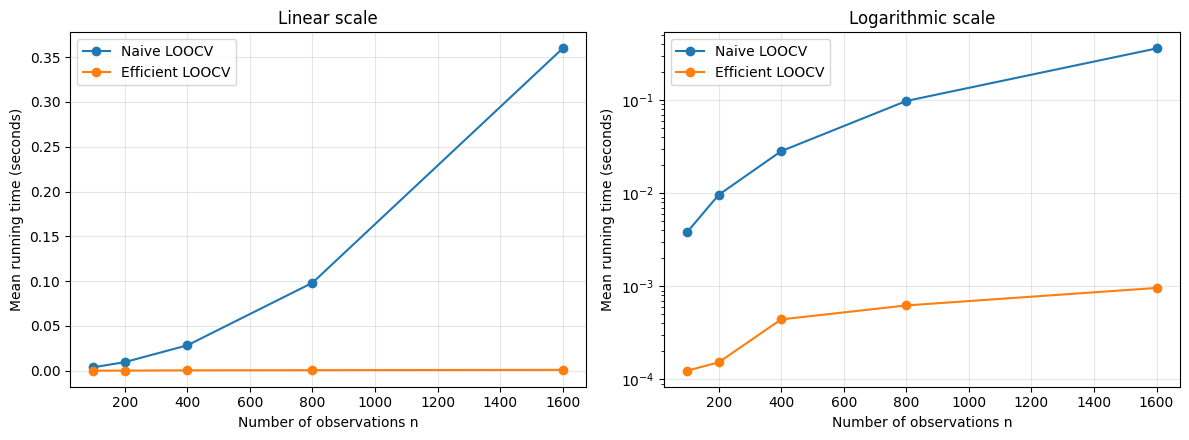
\includegraphics[width=\textwidth]{output.png}
    \caption{Mean running times of the naive and efficient LOOCV
    implementations. The left panel uses a linear scale and the right panel
    uses a logarithmic scale.}
    \label{fig:loocv-running-times}
\end{figure}

Figure~\ref{fig:loocv-running-times} confirms the theoretical complexity
comparison. The naive running time increases rapidly with $n$, whereas the
efficient method remains below one millisecond in this experiment. At
$n=1600$, the naive method takes approximately $0.360$ seconds and the
efficient method approximately $0.000962$ seconds, corresponding to a speed-up
of about $374$.

% =========================================================
% CONCLUSION
% =========================================================
\section{Conclusion}

This practical work illustrates how linear-algebra identities can eliminate
redundant computation. The OLS implementation based on the normal equations
agrees with scikit-learn to numerical precision. The fitted residuals satisfy
$X^\top\epshat\approx\bm0$, as required by the normal equations.

The main theoretical identity is

\[
    \boxed{
    \widehat\varepsilon_i^{(i)}
    =\frac{\widehat\varepsilon_i}{1-h_{ii}}
    }.
\]

It transforms LOOCV from $n$ separate regressions into a single OLS fit followed
by inexpensive leverage corrections. The naive and efficient residuals agree
to approximately $3\times10^{-13}$, while the timing experiment shows an
increasing computational advantage for the efficient method as the sample size
grows.

\end{document}
